\documentclass[letterpaper]{article}
\usepackage[margin=0mm]{geometry}
\usepackage[T1]{fontenc}
\usepackage{lmodern}\pdfmapfile{+lm.map}\pdfmapfile{+cm.map}
\renewcommand{\familydefault}{\sfdefault}
\usepackage{tikz}
\usetikzlibrary{calc}
\pagestyle{empty}
\setlength{\parindent}{0pt}
\begin{document}
\null\begin{tikzpicture}[remember picture,overlay,x=1mm,y=-1mm]
\begin{scope}[shift={(current page.north west)}]
\node[anchor=north west,inner sep=0pt,align=left,font=\fontsize{11}{13.75}\selectfont] at (14,12) {Week 11 / Chip-firing with a sink / Grades 4--5};
\node[anchor=north west,inner sep=0pt,align=left,font=\fontsize{9.5}{11.875}\selectfont] at (14,267) {Bellingham Math Circle / Week 11 / F11-45-v3};
\node[anchor=north east,inner sep=0pt,align=left,font=\fontsize{9.5}{11.875}\selectfont] at (202,267) {1};
\node[anchor=north west,inner sep=0pt,align=left, text width=188mm,font=\fontsize{11.5}{14}\selectfont] at (14,25) {A circle needs one chip for every line touching it before it can share. To share, send one chip along each line. The sink keeps its chips and never shares. Choose one circle at a time. Stop when no circle can share. Empty the sink before each new start. Write each sharing letter in order, then the final piles.};
\node[anchor=north west,inner sep=0pt,align=left, text width=188mm,font=\fontsize{12.5}{16}\selectfont] at (14,56) {\textbf{Problem 1:} Finish each start in two different orders, if possible. After stopping, count each letter in the sharing word. For the same start, can the final piles agree while the sharing counts differ?};
\node[draw,line width=0.9pt,circle,minimum size=44mm,inner sep=0pt] (A) at (61,109) {};
\node[draw,line width=0.9pt,circle,minimum size=44mm,inner sep=0pt] (B) at (155,109) {};
\node[draw,line width=0.9pt,rectangle,minimum width=60mm,minimum height=60mm,inner sep=0pt] (S) at (108,171) {};
\draw[line width=1.05pt] (A) -- (B);
\draw[line width=1.05pt] (A) -- (S);
\draw[line width=1.05pt] (B) -- (S);
\node[anchor=center,inner sep=0pt,align=left,font=\fontsize{14}{17.5}\selectfont] at (61,82) {A};
\node[anchor=center,inner sep=0pt,align=left,font=\fontsize{14}{17.5}\selectfont] at (155,82) {B};
\node[anchor=center,inner sep=0pt,align=left,font=\fontsize{12}{15.0}\selectfont] at (108,194) {SINK};
\node[anchor=north west,inner sep=0pt,align=left, text width=60mm,font=\fontsize{11.5}{14}\selectfont] at (14,148) {A, then B, then A:};
\node[anchor=north west,inner sep=0pt,align=left, text width=60mm,font=\fontsize{11.5}{14}\selectfont] at (14,158) {$\mathrm{A}\;\to\;\mathrm{AB}\;\to\;\mathrm{ABA}$};
\node[anchor=north west,inner sep=0pt,align=left, text width=59mm,font=\fontsize{11.5}{14}\selectfont] at (143,148) {After stopping, count letters: ABA has two A's and one B.};
\draw[black!45,line width=.35pt] (18,207) -- (18,260.0);
\draw[black!45,line width=.35pt] (42,207) -- (42,260.0);
\draw[black!45,line width=.35pt] (66,207) -- (66,260.0);
\draw[black!45,line width=.35pt] (142,207) -- (142,260.0);
\draw[black!45,line width=.35pt] (170,207) -- (170,260.0);
\draw[black!45,line width=.35pt] (198,207) -- (198,260.0);
\draw[black!45,line width=.35pt] (18,207) -- (198,207);
\draw[black!45,line width=.35pt] (18,216) -- (198,216);
\draw[black!45,line width=.35pt] (18,221.5) -- (198,221.5);
\draw[black!45,line width=.35pt] (18,227.0) -- (198,227.0);
\draw[black!45,line width=.35pt] (18,232.5) -- (198,232.5);
\draw[black!45,line width=.35pt] (18,238.0) -- (198,238.0);
\draw[black!45,line width=.35pt] (18,243.5) -- (198,243.5);
\draw[black!45,line width=.35pt] (18,249.0) -- (198,249.0);
\draw[black!45,line width=.35pt] (18,254.5) -- (198,254.5);
\draw[black!45,line width=.35pt] (18,260.0) -- (198,260.0);
\node[anchor=center,inner sep=0pt,align=center,font=\fontsize{10.5}{13.125}\selectfont] at (30.0,211.5) {Start A};
\node[anchor=center,inner sep=0pt,align=center,font=\fontsize{10.5}{13.125}\selectfont] at (54.0,211.5) {Start B};
\node[anchor=center,inner sep=0pt,align=center,font=\fontsize{10.5}{13.125}\selectfont] at (104.0,211.5) {Sharing word};
\node[anchor=center,inner sep=0pt,align=center,font=\fontsize{10.5}{13.125}\selectfont] at (156.0,211.5) {Finish A};
\node[anchor=center,inner sep=0pt,align=center,font=\fontsize{10.5}{13.125}\selectfont] at (184.0,211.5) {Finish B};
\node[anchor=center,inner sep=0pt,align=center,font=\fontsize{10.5}{13.125}\selectfont] at (30.0,218.75) {2};
\node[anchor=center,inner sep=0pt,align=center,font=\fontsize{10.5}{13.125}\selectfont] at (54.0,218.75) {2};
\node[anchor=center,inner sep=0pt,align=center,font=\fontsize{10.5}{13.125}\selectfont] at (104.0,218.75) {};
\node[anchor=center,inner sep=0pt,align=center,font=\fontsize{10.5}{13.125}\selectfont] at (156.0,218.75) {};
\node[anchor=center,inner sep=0pt,align=center,font=\fontsize{10.5}{13.125}\selectfont] at (184.0,218.75) {};
\node[anchor=center,inner sep=0pt,align=center,font=\fontsize{10.5}{13.125}\selectfont] at (30.0,224.25) {2};
\node[anchor=center,inner sep=0pt,align=center,font=\fontsize{10.5}{13.125}\selectfont] at (54.0,224.25) {2};
\node[anchor=center,inner sep=0pt,align=center,font=\fontsize{10.5}{13.125}\selectfont] at (104.0,224.25) {};
\node[anchor=center,inner sep=0pt,align=center,font=\fontsize{10.5}{13.125}\selectfont] at (156.0,224.25) {};
\node[anchor=center,inner sep=0pt,align=center,font=\fontsize{10.5}{13.125}\selectfont] at (184.0,224.25) {};
\node[anchor=center,inner sep=0pt,align=center,font=\fontsize{10.5}{13.125}\selectfont] at (30.0,229.75) {4};
\node[anchor=center,inner sep=0pt,align=center,font=\fontsize{10.5}{13.125}\selectfont] at (54.0,229.75) {0};
\node[anchor=center,inner sep=0pt,align=center,font=\fontsize{10.5}{13.125}\selectfont] at (104.0,229.75) {};
\node[anchor=center,inner sep=0pt,align=center,font=\fontsize{10.5}{13.125}\selectfont] at (156.0,229.75) {};
\node[anchor=center,inner sep=0pt,align=center,font=\fontsize{10.5}{13.125}\selectfont] at (184.0,229.75) {};
\node[anchor=center,inner sep=0pt,align=center,font=\fontsize{10.5}{13.125}\selectfont] at (30.0,235.25) {4};
\node[anchor=center,inner sep=0pt,align=center,font=\fontsize{10.5}{13.125}\selectfont] at (54.0,235.25) {0};
\node[anchor=center,inner sep=0pt,align=center,font=\fontsize{10.5}{13.125}\selectfont] at (104.0,235.25) {};
\node[anchor=center,inner sep=0pt,align=center,font=\fontsize{10.5}{13.125}\selectfont] at (156.0,235.25) {};
\node[anchor=center,inner sep=0pt,align=center,font=\fontsize{10.5}{13.125}\selectfont] at (184.0,235.25) {};
\node[anchor=center,inner sep=0pt,align=center,font=\fontsize{10.5}{13.125}\selectfont] at (30.0,240.75) {3};
\node[anchor=center,inner sep=0pt,align=center,font=\fontsize{10.5}{13.125}\selectfont] at (54.0,240.75) {3};
\node[anchor=center,inner sep=0pt,align=center,font=\fontsize{10.5}{13.125}\selectfont] at (104.0,240.75) {};
\node[anchor=center,inner sep=0pt,align=center,font=\fontsize{10.5}{13.125}\selectfont] at (156.0,240.75) {};
\node[anchor=center,inner sep=0pt,align=center,font=\fontsize{10.5}{13.125}\selectfont] at (184.0,240.75) {};
\node[anchor=center,inner sep=0pt,align=center,font=\fontsize{10.5}{13.125}\selectfont] at (30.0,246.25) {3};
\node[anchor=center,inner sep=0pt,align=center,font=\fontsize{10.5}{13.125}\selectfont] at (54.0,246.25) {3};
\node[anchor=center,inner sep=0pt,align=center,font=\fontsize{10.5}{13.125}\selectfont] at (104.0,246.25) {};
\node[anchor=center,inner sep=0pt,align=center,font=\fontsize{10.5}{13.125}\selectfont] at (156.0,246.25) {};
\node[anchor=center,inner sep=0pt,align=center,font=\fontsize{10.5}{13.125}\selectfont] at (184.0,246.25) {};
\node[anchor=center,inner sep=0pt,align=center,font=\fontsize{10.5}{13.125}\selectfont] at (30.0,251.75) {5};
\node[anchor=center,inner sep=0pt,align=center,font=\fontsize{10.5}{13.125}\selectfont] at (54.0,251.75) {4};
\node[anchor=center,inner sep=0pt,align=center,font=\fontsize{10.5}{13.125}\selectfont] at (104.0,251.75) {};
\node[anchor=center,inner sep=0pt,align=center,font=\fontsize{10.5}{13.125}\selectfont] at (156.0,251.75) {};
\node[anchor=center,inner sep=0pt,align=center,font=\fontsize{10.5}{13.125}\selectfont] at (184.0,251.75) {};
\node[anchor=center,inner sep=0pt,align=center,font=\fontsize{10.5}{13.125}\selectfont] at (30.0,257.25) {5};
\node[anchor=center,inner sep=0pt,align=center,font=\fontsize{10.5}{13.125}\selectfont] at (54.0,257.25) {4};
\node[anchor=center,inner sep=0pt,align=center,font=\fontsize{10.5}{13.125}\selectfont] at (104.0,257.25) {};
\node[anchor=center,inner sep=0pt,align=center,font=\fontsize{10.5}{13.125}\selectfont] at (156.0,257.25) {};
\node[anchor=center,inner sep=0pt,align=center,font=\fontsize{10.5}{13.125}\selectfont] at (184.0,257.25) {};
\end{scope}\end{tikzpicture}\newpage
\null\begin{tikzpicture}[remember picture,overlay,x=1mm,y=-1mm]
\begin{scope}[shift={(current page.north west)}]
\node[anchor=north west,inner sep=0pt,align=left,font=\fontsize{11}{13.75}\selectfont] at (14,12) {Week 11 / Chip-firing with a sink / Grades 4--5};
\node[anchor=north west,inner sep=0pt,align=left,font=\fontsize{9.5}{11.875}\selectfont] at (14,267) {Bellingham Math Circle / Week 11 / F11-45-v3};
\node[anchor=north east,inner sep=0pt,align=left,font=\fontsize{9.5}{11.875}\selectfont] at (202,267) {2};
\node[anchor=north west,inner sep=0pt,align=left, text width=188mm,font=\fontsize{12.5}{16}\selectfont] at (14,26) {\textbf{Problem 2:} Start empty. For each pair of batches, compare adding them together with finishing one before adding the other. Try both batch orders. Does the timing of additions change the finish?};
\node[draw,line width=0.9pt,circle,minimum size=44mm,inner sep=0pt] (A) at (61,80) {};
\node[draw,line width=0.9pt,circle,minimum size=44mm,inner sep=0pt] (B) at (155,80) {};
\node[draw,line width=0.9pt,circle,minimum size=44mm,inner sep=0pt] (C) at (155,162) {};
\node[draw,line width=0.9pt,rectangle,minimum width=60mm,minimum height=60mm,inner sep=0pt] (S) at (61,162) {};
\draw[line width=1.05pt] (S) -- (A);
\draw[line width=1.05pt] (A) -- (B);
\draw[line width=1.05pt] (B) -- (C);
\draw[line width=1.05pt] (C) -- (S);
\node[anchor=center,inner sep=0pt,align=left,font=\fontsize{14}{17.5}\selectfont] at (61,53) {A};
\node[anchor=center,inner sep=0pt,align=left,font=\fontsize{14}{17.5}\selectfont] at (155,53) {B};
\node[anchor=center,inner sep=0pt,align=left,font=\fontsize{14}{17.5}\selectfont] at (183,162) {C};
\node[anchor=center,inner sep=0pt,align=left,font=\fontsize{12}{15.0}\selectfont] at (61,185) {SINK};
\draw[black!45,line width=.35pt] (13,201) -- (13,260);
\draw[black!45,line width=.35pt] (46,201) -- (46,260);
\draw[black!45,line width=.35pt] (79,201) -- (79,260);
\draw[black!45,line width=.35pt] (120,201) -- (120,260);
\draw[black!45,line width=.35pt] (147,201) -- (147,260);
\draw[black!45,line width=.35pt] (174,201) -- (174,260);
\draw[black!45,line width=.35pt] (201,201) -- (201,260);
\draw[black!45,line width=.35pt] (13,201) -- (201,201);
\draw[black!45,line width=.35pt] (13,212) -- (201,212);
\draw[black!45,line width=.35pt] (13,220) -- (201,220);
\draw[black!45,line width=.35pt] (13,228) -- (201,228);
\draw[black!45,line width=.35pt] (13,236) -- (201,236);
\draw[black!45,line width=.35pt] (13,244) -- (201,244);
\draw[black!45,line width=.35pt] (13,252) -- (201,252);
\draw[black!45,line width=.35pt] (13,260) -- (201,260);
\node[anchor=center,inner sep=0pt,align=center,font=\fontsize{9.7}{12.125}\selectfont] at (29.5,206.5) {First batch};
\node[anchor=center,inner sep=0pt,align=center,font=\fontsize{9.7}{12.125}\selectfont] at (62.5,206.5) {Second batch};
\node[anchor=center,inner sep=0pt,align=center,font=\fontsize{9.7}{12.125}\selectfont] at (99.5,206.5) {Timing};
\node[anchor=center,inner sep=0pt,align=center,font=\fontsize{9.7}{12.125}\selectfont] at (133.5,206.5) {Finish A};
\node[anchor=center,inner sep=0pt,align=center,font=\fontsize{9.7}{12.125}\selectfont] at (160.5,206.5) {Finish B};
\node[anchor=center,inner sep=0pt,align=center,font=\fontsize{9.7}{12.125}\selectfont] at (187.5,206.5) {Finish C};
\node[anchor=center,inner sep=0pt,align=center,font=\fontsize{9.7}{12.125}\selectfont] at (29.5,216.0) {4 at B};
\node[anchor=center,inner sep=0pt,align=center,font=\fontsize{9.7}{12.125}\selectfont] at (62.5,216.0) {2 at A};
\node[anchor=center,inner sep=0pt,align=center,font=\fontsize{9.7}{12.125}\selectfont] at (99.5,216.0) {together};
\node[anchor=center,inner sep=0pt,align=center,font=\fontsize{9.7}{12.125}\selectfont] at (133.5,216.0) {};
\node[anchor=center,inner sep=0pt,align=center,font=\fontsize{9.7}{12.125}\selectfont] at (160.5,216.0) {};
\node[anchor=center,inner sep=0pt,align=center,font=\fontsize{9.7}{12.125}\selectfont] at (187.5,216.0) {};
\node[anchor=center,inner sep=0pt,align=center,font=\fontsize{9.7}{12.125}\selectfont] at (29.5,224.0) {4 at B};
\node[anchor=center,inner sep=0pt,align=center,font=\fontsize{9.7}{12.125}\selectfont] at (62.5,224.0) {2 at A};
\node[anchor=center,inner sep=0pt,align=center,font=\fontsize{9.7}{12.125}\selectfont] at (99.5,224.0) {first, then second};
\node[anchor=center,inner sep=0pt,align=center,font=\fontsize{9.7}{12.125}\selectfont] at (133.5,224.0) {};
\node[anchor=center,inner sep=0pt,align=center,font=\fontsize{9.7}{12.125}\selectfont] at (160.5,224.0) {};
\node[anchor=center,inner sep=0pt,align=center,font=\fontsize{9.7}{12.125}\selectfont] at (187.5,224.0) {};
\node[anchor=center,inner sep=0pt,align=center,font=\fontsize{9.7}{12.125}\selectfont] at (29.5,232.0) {4 at B};
\node[anchor=center,inner sep=0pt,align=center,font=\fontsize{9.7}{12.125}\selectfont] at (62.5,232.0) {2 at A};
\node[anchor=center,inner sep=0pt,align=center,font=\fontsize{9.7}{12.125}\selectfont] at (99.5,232.0) {second, then first};
\node[anchor=center,inner sep=0pt,align=center,font=\fontsize{9.7}{12.125}\selectfont] at (133.5,232.0) {};
\node[anchor=center,inner sep=0pt,align=center,font=\fontsize{9.7}{12.125}\selectfont] at (160.5,232.0) {};
\node[anchor=center,inner sep=0pt,align=center,font=\fontsize{9.7}{12.125}\selectfont] at (187.5,232.0) {};
\node[anchor=center,inner sep=0pt,align=center,font=\fontsize{9.7}{12.125}\selectfont] at (29.5,240.0) {3 at A};
\node[anchor=center,inner sep=0pt,align=center,font=\fontsize{9.7}{12.125}\selectfont] at (62.5,240.0) {3 at C};
\node[anchor=center,inner sep=0pt,align=center,font=\fontsize{9.7}{12.125}\selectfont] at (99.5,240.0) {together};
\node[anchor=center,inner sep=0pt,align=center,font=\fontsize{9.7}{12.125}\selectfont] at (133.5,240.0) {};
\node[anchor=center,inner sep=0pt,align=center,font=\fontsize{9.7}{12.125}\selectfont] at (160.5,240.0) {};
\node[anchor=center,inner sep=0pt,align=center,font=\fontsize{9.7}{12.125}\selectfont] at (187.5,240.0) {};
\node[anchor=center,inner sep=0pt,align=center,font=\fontsize{9.7}{12.125}\selectfont] at (29.5,248.0) {3 at A};
\node[anchor=center,inner sep=0pt,align=center,font=\fontsize{9.7}{12.125}\selectfont] at (62.5,248.0) {3 at C};
\node[anchor=center,inner sep=0pt,align=center,font=\fontsize{9.7}{12.125}\selectfont] at (99.5,248.0) {first, then second};
\node[anchor=center,inner sep=0pt,align=center,font=\fontsize{9.7}{12.125}\selectfont] at (133.5,248.0) {};
\node[anchor=center,inner sep=0pt,align=center,font=\fontsize{9.7}{12.125}\selectfont] at (160.5,248.0) {};
\node[anchor=center,inner sep=0pt,align=center,font=\fontsize{9.7}{12.125}\selectfont] at (187.5,248.0) {};
\node[anchor=center,inner sep=0pt,align=center,font=\fontsize{9.7}{12.125}\selectfont] at (29.5,256.0) {3 at A};
\node[anchor=center,inner sep=0pt,align=center,font=\fontsize{9.7}{12.125}\selectfont] at (62.5,256.0) {3 at C};
\node[anchor=center,inner sep=0pt,align=center,font=\fontsize{9.7}{12.125}\selectfont] at (99.5,256.0) {second, then first};
\node[anchor=center,inner sep=0pt,align=center,font=\fontsize{9.7}{12.125}\selectfont] at (133.5,256.0) {};
\node[anchor=center,inner sep=0pt,align=center,font=\fontsize{9.7}{12.125}\selectfont] at (160.5,256.0) {};
\node[anchor=center,inner sep=0pt,align=center,font=\fontsize{9.7}{12.125}\selectfont] at (187.5,256.0) {};
\end{scope}\end{tikzpicture}\newpage
\null\begin{tikzpicture}[remember picture,overlay,x=1mm,y=-1mm]
\begin{scope}[shift={(current page.north west)}]
\node[anchor=north west,inner sep=0pt,align=left,font=\fontsize{11}{13.75}\selectfont] at (14,12) {Week 11 / Chip-firing with a sink / Grades 4--5};
\node[anchor=north west,inner sep=0pt,align=left,font=\fontsize{9.5}{11.875}\selectfont] at (14,267) {Bellingham Math Circle / Week 11 / F11-45-v3};
\node[anchor=north east,inner sep=0pt,align=left,font=\fontsize{9.5}{11.875}\selectfont] at (202,267) {3};
\node[anchor=north west,inner sep=0pt,align=left, text width=188mm,font=\fontsize{12.5}{16}\selectfont] at (14,26) {\textbf{Problem 3:} From each start, repeatedly add one chip to A and finish after each addition. Record the pairs you get. Which starts return to themselves? Can two different starts give the same pair after one addition?};
\node[draw,line width=0.9pt,circle,minimum size=44mm,inner sep=0pt] (A) at (61,86) {};
\node[draw,line width=0.9pt,circle,minimum size=44mm,inner sep=0pt] (B) at (155,86) {};
\node[draw,line width=0.9pt,rectangle,minimum width=60mm,minimum height=60mm,inner sep=0pt] (S) at (108,148) {};
\draw[line width=1.05pt] (A) -- (B);
\draw[line width=1.05pt] (A) -- (S);
\draw[line width=1.05pt] (B) -- (S);
\node[anchor=center,inner sep=0pt,align=left,font=\fontsize{14}{17.5}\selectfont] at (61,59) {A};
\node[anchor=center,inner sep=0pt,align=left,font=\fontsize{14}{17.5}\selectfont] at (155,59) {B};
\node[anchor=center,inner sep=0pt,align=left,font=\fontsize{12}{15.0}\selectfont] at (108,171) {SINK};
\draw[black!45,line width=.35pt] (17,192) -- (17,241);
\draw[black!45,line width=.35pt] (40,192) -- (40,241);
\draw[black!45,line width=.35pt] (63,192) -- (63,241);
\draw[black!45,line width=.35pt] (97,192) -- (97,241);
\draw[black!45,line width=.35pt] (131,192) -- (131,241);
\draw[black!45,line width=.35pt] (165,192) -- (165,241);
\draw[black!45,line width=.35pt] (199,192) -- (199,241);
\draw[black!45,line width=.35pt] (17,192) -- (199,192);
\draw[black!45,line width=.35pt] (17,201) -- (199,201);
\draw[black!45,line width=.35pt] (17,211) -- (199,211);
\draw[black!45,line width=.35pt] (17,221) -- (199,221);
\draw[black!45,line width=.35pt] (17,231) -- (199,231);
\draw[black!45,line width=.35pt] (17,241) -- (199,241);
\node[anchor=center,inner sep=0pt,align=center,font=\fontsize{10.5}{13.125}\selectfont] at (28.5,196.5) {Start A};
\node[anchor=center,inner sep=0pt,align=center,font=\fontsize{10.5}{13.125}\selectfont] at (51.5,196.5) {Start B};
\node[anchor=center,inner sep=0pt,align=center,font=\fontsize{10.5}{13.125}\selectfont] at (80.0,196.5) {After 1};
\node[anchor=center,inner sep=0pt,align=center,font=\fontsize{10.5}{13.125}\selectfont] at (114.0,196.5) {After 2};
\node[anchor=center,inner sep=0pt,align=center,font=\fontsize{10.5}{13.125}\selectfont] at (148.0,196.5) {After 3};
\node[anchor=center,inner sep=0pt,align=center,font=\fontsize{10.5}{13.125}\selectfont] at (182.0,196.5) {After 4};
\node[anchor=center,inner sep=0pt,align=center,font=\fontsize{10.5}{13.125}\selectfont] at (28.5,206.0) {0};
\node[anchor=center,inner sep=0pt,align=center,font=\fontsize{10.5}{13.125}\selectfont] at (51.5,206.0) {0};
\node[anchor=center,inner sep=0pt,align=center,font=\fontsize{10.5}{13.125}\selectfont] at (80.0,206.0) {};
\node[anchor=center,inner sep=0pt,align=center,font=\fontsize{10.5}{13.125}\selectfont] at (114.0,206.0) {};
\node[anchor=center,inner sep=0pt,align=center,font=\fontsize{10.5}{13.125}\selectfont] at (148.0,206.0) {};
\node[anchor=center,inner sep=0pt,align=center,font=\fontsize{10.5}{13.125}\selectfont] at (182.0,206.0) {};
\node[anchor=center,inner sep=0pt,align=center,font=\fontsize{10.5}{13.125}\selectfont] at (28.5,216.0) {1};
\node[anchor=center,inner sep=0pt,align=center,font=\fontsize{10.5}{13.125}\selectfont] at (51.5,216.0) {0};
\node[anchor=center,inner sep=0pt,align=center,font=\fontsize{10.5}{13.125}\selectfont] at (80.0,216.0) {};
\node[anchor=center,inner sep=0pt,align=center,font=\fontsize{10.5}{13.125}\selectfont] at (114.0,216.0) {};
\node[anchor=center,inner sep=0pt,align=center,font=\fontsize{10.5}{13.125}\selectfont] at (148.0,216.0) {};
\node[anchor=center,inner sep=0pt,align=center,font=\fontsize{10.5}{13.125}\selectfont] at (182.0,216.0) {};
\node[anchor=center,inner sep=0pt,align=center,font=\fontsize{10.5}{13.125}\selectfont] at (28.5,226.0) {0};
\node[anchor=center,inner sep=0pt,align=center,font=\fontsize{10.5}{13.125}\selectfont] at (51.5,226.0) {1};
\node[anchor=center,inner sep=0pt,align=center,font=\fontsize{10.5}{13.125}\selectfont] at (80.0,226.0) {};
\node[anchor=center,inner sep=0pt,align=center,font=\fontsize{10.5}{13.125}\selectfont] at (114.0,226.0) {};
\node[anchor=center,inner sep=0pt,align=center,font=\fontsize{10.5}{13.125}\selectfont] at (148.0,226.0) {};
\node[anchor=center,inner sep=0pt,align=center,font=\fontsize{10.5}{13.125}\selectfont] at (182.0,226.0) {};
\node[anchor=center,inner sep=0pt,align=center,font=\fontsize{10.5}{13.125}\selectfont] at (28.5,236.0) {1};
\node[anchor=center,inner sep=0pt,align=center,font=\fontsize{10.5}{13.125}\selectfont] at (51.5,236.0) {1};
\node[anchor=center,inner sep=0pt,align=center,font=\fontsize{10.5}{13.125}\selectfont] at (80.0,236.0) {};
\node[anchor=center,inner sep=0pt,align=center,font=\fontsize{10.5}{13.125}\selectfont] at (114.0,236.0) {};
\node[anchor=center,inner sep=0pt,align=center,font=\fontsize{10.5}{13.125}\selectfont] at (148.0,236.0) {};
\node[anchor=center,inner sep=0pt,align=center,font=\fontsize{10.5}{13.125}\selectfont] at (182.0,236.0) {};
\draw[black!25,line width=.35pt] (14,252) -- (202,252);
\end{scope}\end{tikzpicture}\newpage
\null\begin{tikzpicture}[remember picture,overlay,x=1mm,y=-1mm]
\begin{scope}[shift={(current page.north west)}]
\node[anchor=north west,inner sep=0pt,align=left,font=\fontsize{11}{13.75}\selectfont] at (14,12) {Week 11 / Chip-firing with a sink / Grades 4--5};
\node[anchor=north west,inner sep=0pt,align=left,font=\fontsize{9.5}{11.875}\selectfont] at (14,267) {Bellingham Math Circle / Week 11 / F11-45-v3};
\node[anchor=north east,inner sep=0pt,align=left,font=\fontsize{9.5}{11.875}\selectfont] at (202,267) {4};
\node[anchor=north west,inner sep=0pt,align=left, text width=188mm,font=\fontsize{12.5}{16}\selectfont] at (14,26) {\textbf{Problem 4:} Finish each start in two different orders, if possible. After stopping, compare the final piles and count each letter in the sharing words. Does the extra line change your conclusion about order?};
\node[draw,line width=0.9pt,circle,minimum size=44mm,inner sep=0pt] (A) at (61,78) {};
\node[draw,line width=0.9pt,circle,minimum size=44mm,inner sep=0pt] (B) at (155,78) {};
\node[draw,line width=0.9pt,circle,minimum size=44mm,inner sep=0pt] (C) at (155,160) {};
\node[draw,line width=0.9pt,rectangle,minimum width=60mm,minimum height=60mm,inner sep=0pt] (S) at (61,160) {};
\draw[line width=1.05pt] (S) -- (A);
\draw[line width=1.05pt] (A) -- (B);
\draw[line width=1.05pt] (B) -- (C);
\draw[line width=1.05pt] (C) -- (S);
\draw[line width=1.05pt] (A) -- (C);
\node[anchor=center,inner sep=0pt,align=left,font=\fontsize{14}{17.5}\selectfont] at (61,51) {A};
\node[anchor=center,inner sep=0pt,align=left,font=\fontsize{14}{17.5}\selectfont] at (155,51) {B};
\node[anchor=center,inner sep=0pt,align=left,font=\fontsize{14}{17.5}\selectfont] at (183,160) {C};
\node[anchor=center,inner sep=0pt,align=left,font=\fontsize{12}{15.0}\selectfont] at (61,183) {SINK};
\draw[black!45,line width=.35pt] (13,204) -- (13,258.4);
\draw[black!45,line width=.35pt] (34,204) -- (34,258.4);
\draw[black!45,line width=.35pt] (55,204) -- (55,258.4);
\draw[black!45,line width=.35pt] (76,204) -- (76,258.4);
\draw[black!45,line width=.35pt] (139,204) -- (139,258.4);
\draw[black!45,line width=.35pt] (160,204) -- (160,258.4);
\draw[black!45,line width=.35pt] (181,204) -- (181,258.4);
\draw[black!45,line width=.35pt] (202,204) -- (202,258.4);
\draw[black!45,line width=.35pt] (13,204) -- (202,204);
\draw[black!45,line width=.35pt] (13,214) -- (202,214);
\draw[black!45,line width=.35pt] (13,221.4) -- (202,221.4);
\draw[black!45,line width=.35pt] (13,228.8) -- (202,228.8);
\draw[black!45,line width=.35pt] (13,236.2) -- (202,236.2);
\draw[black!45,line width=.35pt] (13,243.6) -- (202,243.6);
\draw[black!45,line width=.35pt] (13,251.0) -- (202,251.0);
\draw[black!45,line width=.35pt] (13,258.4) -- (202,258.4);
\node[anchor=center,inner sep=0pt,align=center,font=\fontsize{9.2}{11.5}\selectfont] at (23.5,209.0) {Start A};
\node[anchor=center,inner sep=0pt,align=center,font=\fontsize{9.2}{11.5}\selectfont] at (44.5,209.0) {Start B};
\node[anchor=center,inner sep=0pt,align=center,font=\fontsize{9.2}{11.5}\selectfont] at (65.5,209.0) {Start C};
\node[anchor=center,inner sep=0pt,align=center,font=\fontsize{9.2}{11.5}\selectfont] at (107.5,209.0) {Sharing word};
\node[anchor=center,inner sep=0pt,align=center,font=\fontsize{9.2}{11.5}\selectfont] at (149.5,209.0) {End A};
\node[anchor=center,inner sep=0pt,align=center,font=\fontsize{9.2}{11.5}\selectfont] at (170.5,209.0) {End B};
\node[anchor=center,inner sep=0pt,align=center,font=\fontsize{9.2}{11.5}\selectfont] at (191.5,209.0) {End C};
\node[anchor=center,inner sep=0pt,align=center,font=\fontsize{9.2}{11.5}\selectfont] at (23.5,217.7) {3};
\node[anchor=center,inner sep=0pt,align=center,font=\fontsize{9.2}{11.5}\selectfont] at (44.5,217.7) {0};
\node[anchor=center,inner sep=0pt,align=center,font=\fontsize{9.2}{11.5}\selectfont] at (65.5,217.7) {3};
\node[anchor=center,inner sep=0pt,align=center,font=\fontsize{9.2}{11.5}\selectfont] at (107.5,217.7) {};
\node[anchor=center,inner sep=0pt,align=center,font=\fontsize{9.2}{11.5}\selectfont] at (149.5,217.7) {};
\node[anchor=center,inner sep=0pt,align=center,font=\fontsize{9.2}{11.5}\selectfont] at (170.5,217.7) {};
\node[anchor=center,inner sep=0pt,align=center,font=\fontsize{9.2}{11.5}\selectfont] at (191.5,217.7) {};
\node[anchor=center,inner sep=0pt,align=center,font=\fontsize{9.2}{11.5}\selectfont] at (23.5,225.1) {3};
\node[anchor=center,inner sep=0pt,align=center,font=\fontsize{9.2}{11.5}\selectfont] at (44.5,225.1) {0};
\node[anchor=center,inner sep=0pt,align=center,font=\fontsize{9.2}{11.5}\selectfont] at (65.5,225.1) {3};
\node[anchor=center,inner sep=0pt,align=center,font=\fontsize{9.2}{11.5}\selectfont] at (107.5,225.1) {};
\node[anchor=center,inner sep=0pt,align=center,font=\fontsize{9.2}{11.5}\selectfont] at (149.5,225.1) {};
\node[anchor=center,inner sep=0pt,align=center,font=\fontsize{9.2}{11.5}\selectfont] at (170.5,225.1) {};
\node[anchor=center,inner sep=0pt,align=center,font=\fontsize{9.2}{11.5}\selectfont] at (191.5,225.1) {};
\node[anchor=center,inner sep=0pt,align=center,font=\fontsize{9.2}{11.5}\selectfont] at (23.5,232.5) {0};
\node[anchor=center,inner sep=0pt,align=center,font=\fontsize{9.2}{11.5}\selectfont] at (44.5,232.5) {6};
\node[anchor=center,inner sep=0pt,align=center,font=\fontsize{9.2}{11.5}\selectfont] at (65.5,232.5) {0};
\node[anchor=center,inner sep=0pt,align=center,font=\fontsize{9.2}{11.5}\selectfont] at (107.5,232.5) {};
\node[anchor=center,inner sep=0pt,align=center,font=\fontsize{9.2}{11.5}\selectfont] at (149.5,232.5) {};
\node[anchor=center,inner sep=0pt,align=center,font=\fontsize{9.2}{11.5}\selectfont] at (170.5,232.5) {};
\node[anchor=center,inner sep=0pt,align=center,font=\fontsize{9.2}{11.5}\selectfont] at (191.5,232.5) {};
\node[anchor=center,inner sep=0pt,align=center,font=\fontsize{9.2}{11.5}\selectfont] at (23.5,239.9) {0};
\node[anchor=center,inner sep=0pt,align=center,font=\fontsize{9.2}{11.5}\selectfont] at (44.5,239.9) {6};
\node[anchor=center,inner sep=0pt,align=center,font=\fontsize{9.2}{11.5}\selectfont] at (65.5,239.9) {0};
\node[anchor=center,inner sep=0pt,align=center,font=\fontsize{9.2}{11.5}\selectfont] at (107.5,239.9) {};
\node[anchor=center,inner sep=0pt,align=center,font=\fontsize{9.2}{11.5}\selectfont] at (149.5,239.9) {};
\node[anchor=center,inner sep=0pt,align=center,font=\fontsize{9.2}{11.5}\selectfont] at (170.5,239.9) {};
\node[anchor=center,inner sep=0pt,align=center,font=\fontsize{9.2}{11.5}\selectfont] at (191.5,239.9) {};
\node[anchor=center,inner sep=0pt,align=center,font=\fontsize{9.2}{11.5}\selectfont] at (23.5,247.3) {4};
\node[anchor=center,inner sep=0pt,align=center,font=\fontsize{9.2}{11.5}\selectfont] at (44.5,247.3) {1};
\node[anchor=center,inner sep=0pt,align=center,font=\fontsize{9.2}{11.5}\selectfont] at (65.5,247.3) {2};
\node[anchor=center,inner sep=0pt,align=center,font=\fontsize{9.2}{11.5}\selectfont] at (107.5,247.3) {};
\node[anchor=center,inner sep=0pt,align=center,font=\fontsize{9.2}{11.5}\selectfont] at (149.5,247.3) {};
\node[anchor=center,inner sep=0pt,align=center,font=\fontsize{9.2}{11.5}\selectfont] at (170.5,247.3) {};
\node[anchor=center,inner sep=0pt,align=center,font=\fontsize{9.2}{11.5}\selectfont] at (191.5,247.3) {};
\node[anchor=center,inner sep=0pt,align=center,font=\fontsize{9.2}{11.5}\selectfont] at (23.5,254.7) {4};
\node[anchor=center,inner sep=0pt,align=center,font=\fontsize{9.2}{11.5}\selectfont] at (44.5,254.7) {1};
\node[anchor=center,inner sep=0pt,align=center,font=\fontsize{9.2}{11.5}\selectfont] at (65.5,254.7) {2};
\node[anchor=center,inner sep=0pt,align=center,font=\fontsize{9.2}{11.5}\selectfont] at (107.5,254.7) {};
\node[anchor=center,inner sep=0pt,align=center,font=\fontsize{9.2}{11.5}\selectfont] at (149.5,254.7) {};
\node[anchor=center,inner sep=0pt,align=center,font=\fontsize{9.2}{11.5}\selectfont] at (170.5,254.7) {};
\node[anchor=center,inner sep=0pt,align=center,font=\fontsize{9.2}{11.5}\selectfont] at (191.5,254.7) {};
\end{scope}\end{tikzpicture}\newpage
\null\begin{tikzpicture}[remember picture,overlay,x=1mm,y=-1mm]
\begin{scope}[shift={(current page.north west)}]
\node[anchor=north west,inner sep=0pt,align=left,font=\fontsize{11}{13.75}\selectfont] at (14,12) {Week 11 / Chip-firing with a sink / Grades 4--5};
\node[anchor=north west,inner sep=0pt,align=left,font=\fontsize{9.5}{11.875}\selectfont] at (14,267) {Bellingham Math Circle / Week 11 / F11-45-v3};
\node[anchor=north east,inner sep=0pt,align=left,font=\fontsize{9.5}{11.875}\selectfont] at (202,267) {5};
\node[anchor=north west,inner sep=0pt,align=left, text width=188mm,font=\fontsize{12.5}{16}\selectfont] at (14,26) {\textbf{Problem 5:} Try starts with all 12 chips at B, with 6 at A and 6 at C, and with 4 at each circle. Could any order of sharing continue forever? Explain why sharing must stop for any finite number of chips on this board.};
\node[draw,line width=0.9pt,circle,minimum size=44mm,inner sep=0pt] (A) at (61,87) {};
\node[draw,line width=0.9pt,circle,minimum size=44mm,inner sep=0pt] (B) at (155,87) {};
\node[draw,line width=0.9pt,circle,minimum size=44mm,inner sep=0pt] (C) at (155,169) {};
\node[draw,line width=0.9pt,rectangle,minimum width=60mm,minimum height=60mm,inner sep=0pt] (S) at (61,169) {};
\draw[line width=1.05pt] (S) -- (A);
\draw[line width=1.05pt] (A) -- (B);
\draw[line width=1.05pt] (B) -- (C);
\draw[line width=1.05pt] (C) -- (S);
\node[anchor=center,inner sep=0pt,align=left,font=\fontsize{14}{17.5}\selectfont] at (61,60) {A};
\node[anchor=center,inner sep=0pt,align=left,font=\fontsize{14}{17.5}\selectfont] at (155,60) {B};
\node[anchor=center,inner sep=0pt,align=left,font=\fontsize{14}{17.5}\selectfont] at (183,169) {C};
\node[anchor=center,inner sep=0pt,align=left,font=\fontsize{12}{15.0}\selectfont] at (61,192) {SINK};
\draw[black!25,line width=.35pt] (14,220) -- (202,220);
\draw[black!25,line width=.35pt] (14,231) -- (202,231);
\draw[black!25,line width=.35pt] (14,242) -- (202,242);
\draw[black!25,line width=.35pt] (14,253) -- (202,253);
\end{scope}\end{tikzpicture}\newpage
\null\begin{tikzpicture}[remember picture,overlay,x=1mm,y=-1mm]
\begin{scope}[shift={(current page.north west)}]
\node[anchor=north west,inner sep=0pt,align=left,font=\fontsize{11}{13.75}\selectfont] at (14,12) {Week 11 / Chip-firing with a sink / Grades 4--5};
\node[anchor=north west,inner sep=0pt,align=left,font=\fontsize{9.5}{11.875}\selectfont] at (14,267) {Bellingham Math Circle / Week 11 / F11-45-v3};
\node[anchor=north east,inner sep=0pt,align=left,font=\fontsize{9.5}{11.875}\selectfont] at (202,267) {6};
\node[anchor=north west,inner sep=0pt,align=left, text width=188mm,font=\fontsize{12.5}{16}\selectfont] at (14,26) {\textbf{Problem 6:} Start with 8 chips at B and none at A or C. Find two different orders that finish. Explain why every order must give the same final piles and sharing counts, for this start and for any other start on this board.};
\node[draw,line width=0.9pt,circle,minimum size=44mm,inner sep=0pt] (A) at (61,86) {};
\node[draw,line width=0.9pt,circle,minimum size=44mm,inner sep=0pt] (B) at (155,86) {};
\node[draw,line width=0.9pt,circle,minimum size=44mm,inner sep=0pt] (C) at (155,168) {};
\node[draw,line width=0.9pt,rectangle,minimum width=60mm,minimum height=60mm,inner sep=0pt] (S) at (61,168) {};
\draw[line width=1.05pt] (S) -- (A);
\draw[line width=1.05pt] (A) -- (B);
\draw[line width=1.05pt] (B) -- (C);
\draw[line width=1.05pt] (C) -- (S);
\node[anchor=center,inner sep=0pt,align=left,font=\fontsize{14}{17.5}\selectfont] at (61,59) {A};
\node[anchor=center,inner sep=0pt,align=left,font=\fontsize{14}{17.5}\selectfont] at (155,59) {B};
\node[anchor=center,inner sep=0pt,align=left,font=\fontsize{14}{17.5}\selectfont] at (183,168) {C};
\node[anchor=center,inner sep=0pt,align=left,font=\fontsize{12}{15.0}\selectfont] at (61,191) {SINK};
\draw[black!25,line width=.35pt] (14,216) -- (202,216);
\draw[black!25,line width=.35pt] (14,228) -- (202,228);
\draw[black!25,line width=.35pt] (14,240) -- (202,240);
\draw[black!25,line width=.35pt] (14,252) -- (202,252);
\end{scope}\end{tikzpicture}
\end{document}
